\section{Results} \label{sec:results}

\TODO{To demonstrate the simplicity of deploying pytokio on different Cray systems, results from both NERSC's Cori and ALCF's Theta systems will also be presented.}

\subsection{Analysis for users \& administrators} \label{sec:results/users}

\begin{figure}
    \centering
    \begin{subfigure}{0.55\textwidth}
    	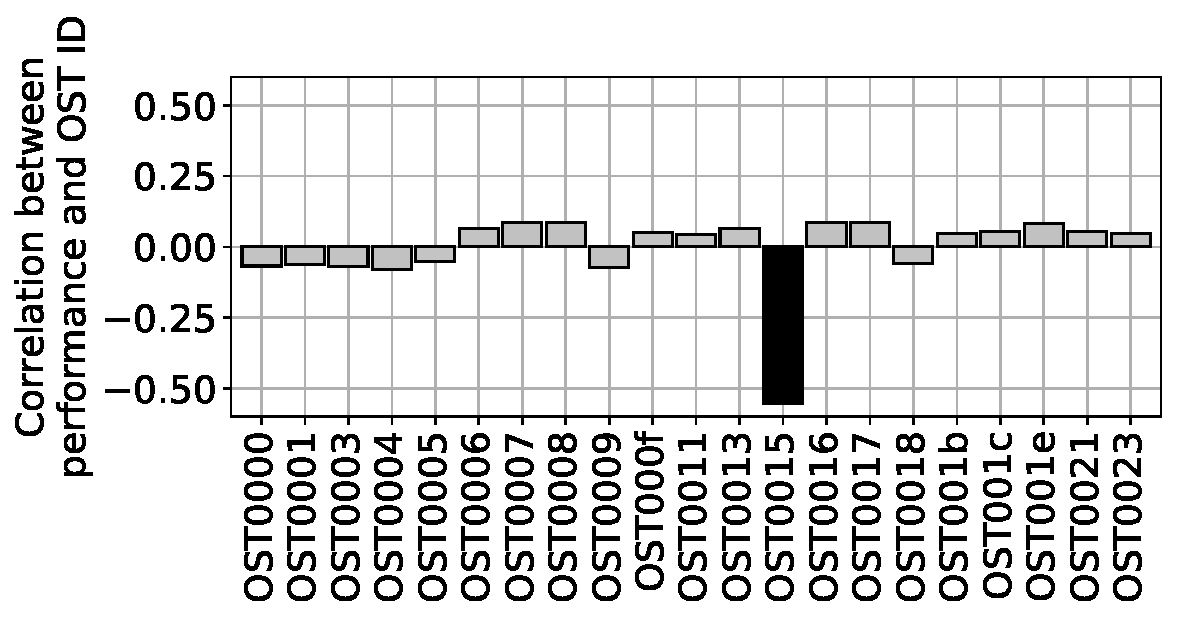
\includegraphics[width=0.9\linewidth]{darshan_bad_ost}
        \caption{Correlation between I/O performance and Lustre OST}
        \label{fig:stragging-ost/correlation}
    \end{subfigure}
    \begin{subfigure}{0.55\textwidth}
    	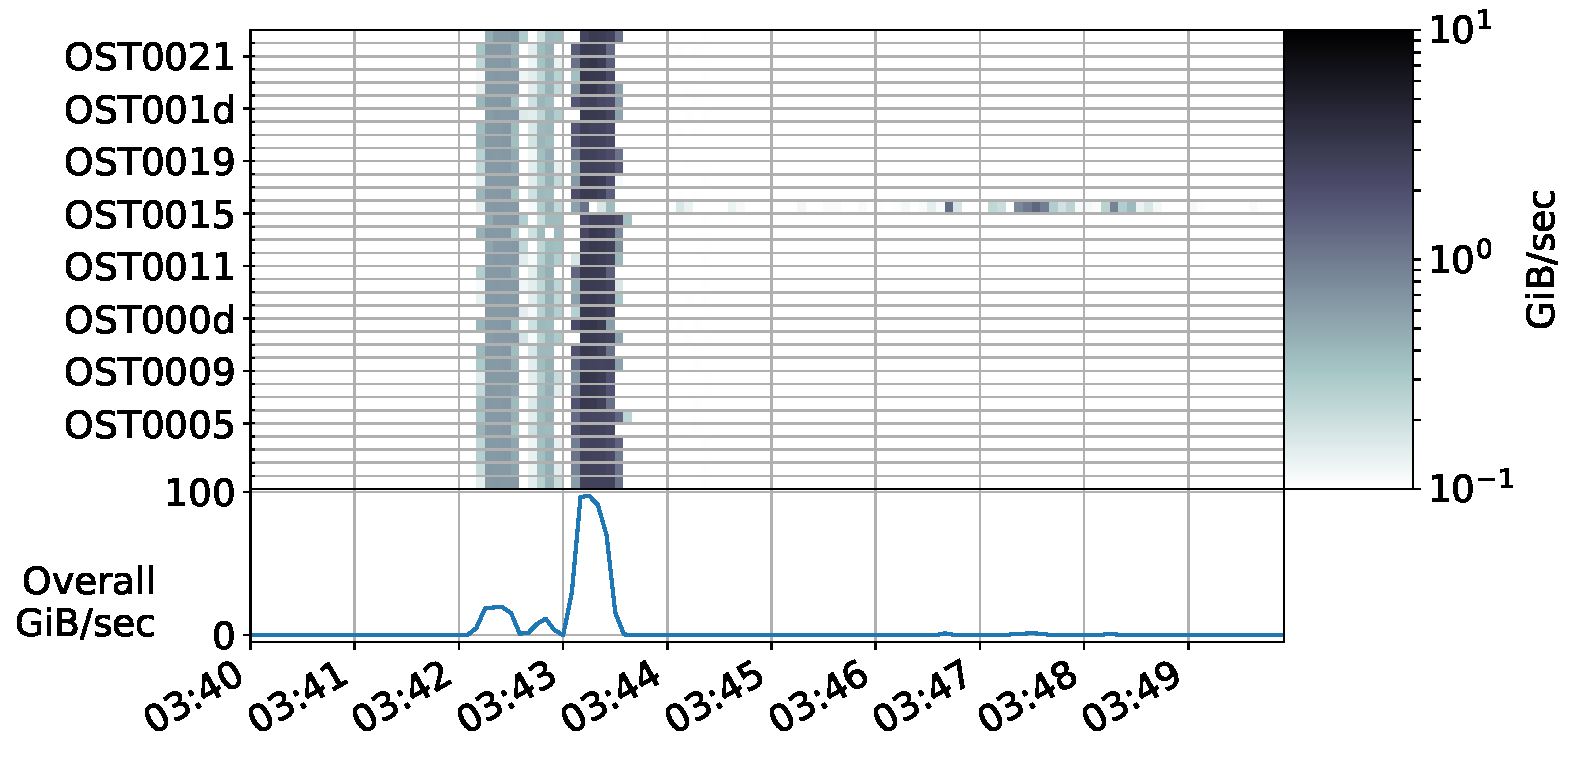
\includegraphics[width=0.9\linewidth]{heatmap_straggler}
        \caption{Per-OST performance over time}
        \label{fig:stragging-ost/heatmap}
    \end{subfigure}
    %\vspace{-.3in}
    \caption{(a) Correlation between per-file application I/O performance and the OSTs to which each file was mapped (from Darshan); shading indicates statistical significance, with darker bars being more significant.
    (b) Per-OST I/O performance measured over the same time that the job in (a) was running (from LMT).
    In both (a) and (b), OST0015 is identified as showing abnormally poor performance.
    }
    \label{fig:straggling-ost}
    \vspace{-.2in}
\end{figure}

Answering the question of why I/O for a user's job was slow was one of the principal motivators behind developing pytokio, and the UMAMI approach described in Section \ref{sec:apps/analysis} goes a long way towards answering this question.
In the absence of a series of jobs with similar I/O from which an UMAMI diagram can be assembled, though, the \texttt{summarize\_job} tool can still provide useful metrics such the degree to which the user's job experienced I/O contention with others (its coverage factor).

In the absence of I/O contention being reported by \texttt{summarize\_job}, pytokio's Darshan connector provides a simple way to connect the output of different Darshan modules~\cite{Snyder2016modular} with powerful statistical analyses such as those provided by SciPy.

For example, pytokio includes a \texttt{darshan\_bad\_ost} analysis tool which tabulates the bytes read and written to each file profiled by Darshan in a Darshan log, then divides this by the total time the application spent performing I/O that file to obtain an estimate of that file's I/O performance.
It then uses data from Darshan's Lustre module to map these performance estimates to the OSTs over which each file was striped.
Given enough files spread across subsets of the file system's OSTs, it is able to calculate the Pearson correlation coefficients between estimated I/O performance and individual OSTs.

Figure \ref{fig:stragging-ost/correlation} shows the results this correlation analysis for a particular slow-running job that performed file-per-process I/O to files with a stripe width of 1.
For almost all OSTs, the correlation between performance and OST ID wavers near zero, indicating minimal correlation.
However, OST0015 stands out in stark contrast; it correlates strongly and negatively with performance and suggests that this OST is in an unhealthy state and not delivering the same level of performance as its peers.
Using data from the LMT connector (shown in Figure \ref{fig:stragging-ost/heatmap}) confirms this.
Whereas almost all OSTs during this job's write phase were able to complete their I/O between 3:43 AM and 3:44 AM, OST0015 shows a long tail of performance, with relatively little I/O activity between 3:43 AM and 3:44 AM, and I/O activity still occurring as late as 3:48 AM.
Using both statistical analysis of Darshan data and a visualization of high-resolution LMT data, the poor performance of this job can be confidently attributed to a poorly performing OST.

% \begin{figure}
%     \centering
%     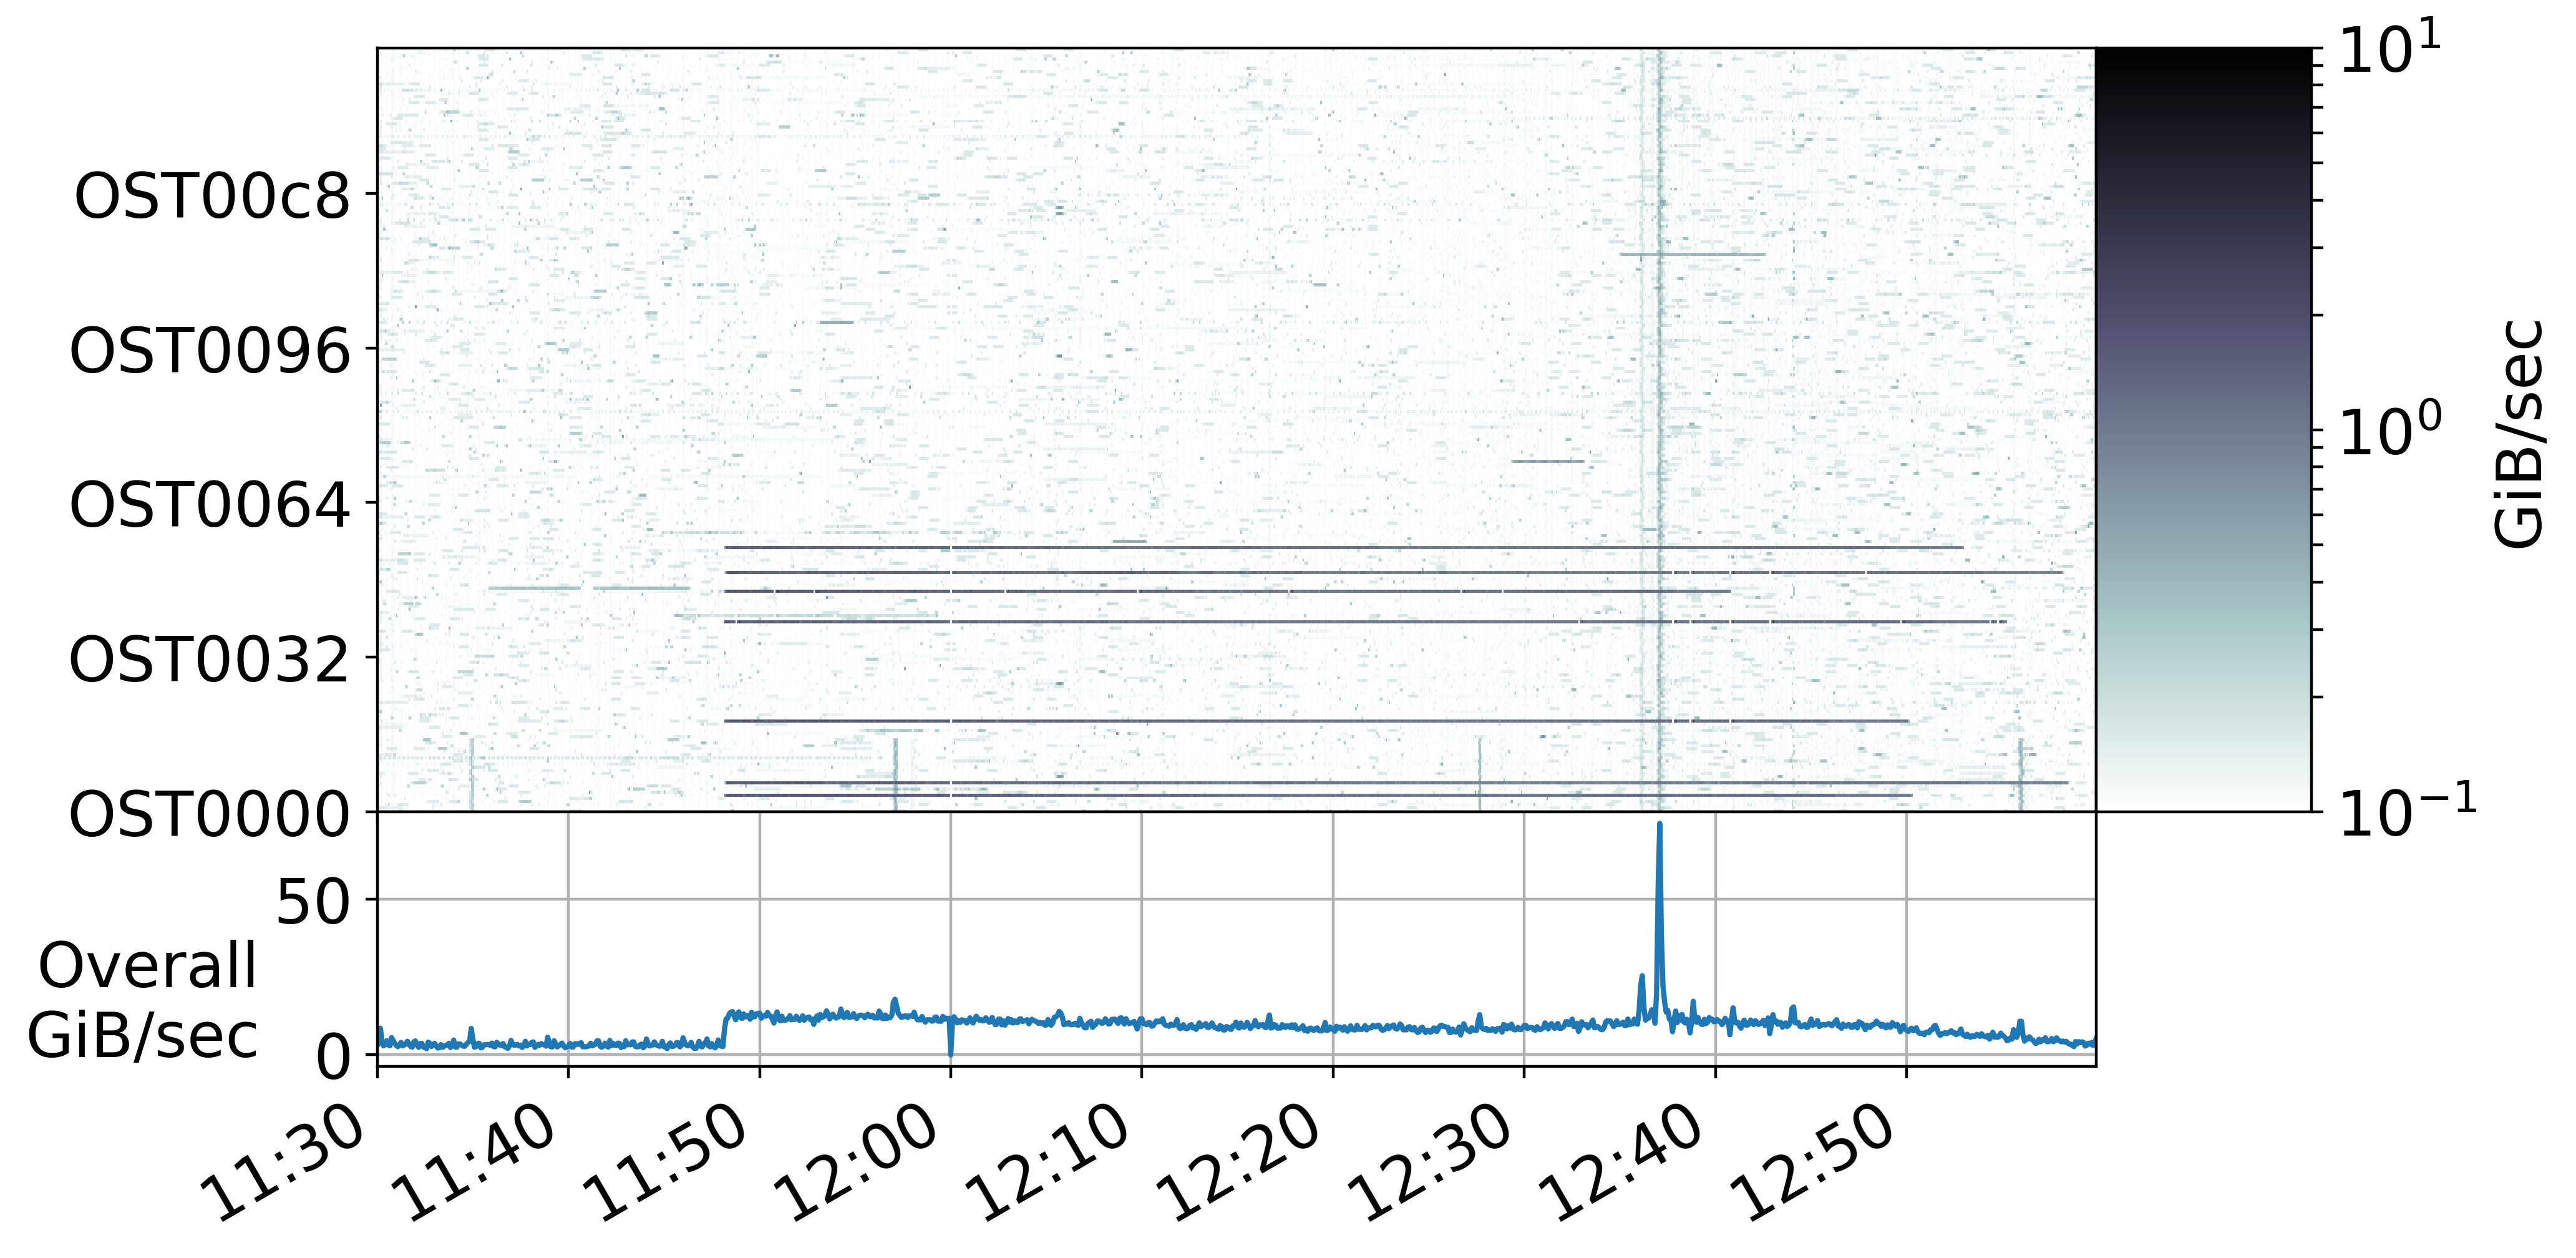
\includegraphics[width=0.9\columnwidth]{heatmap_unoptimized_write}
%     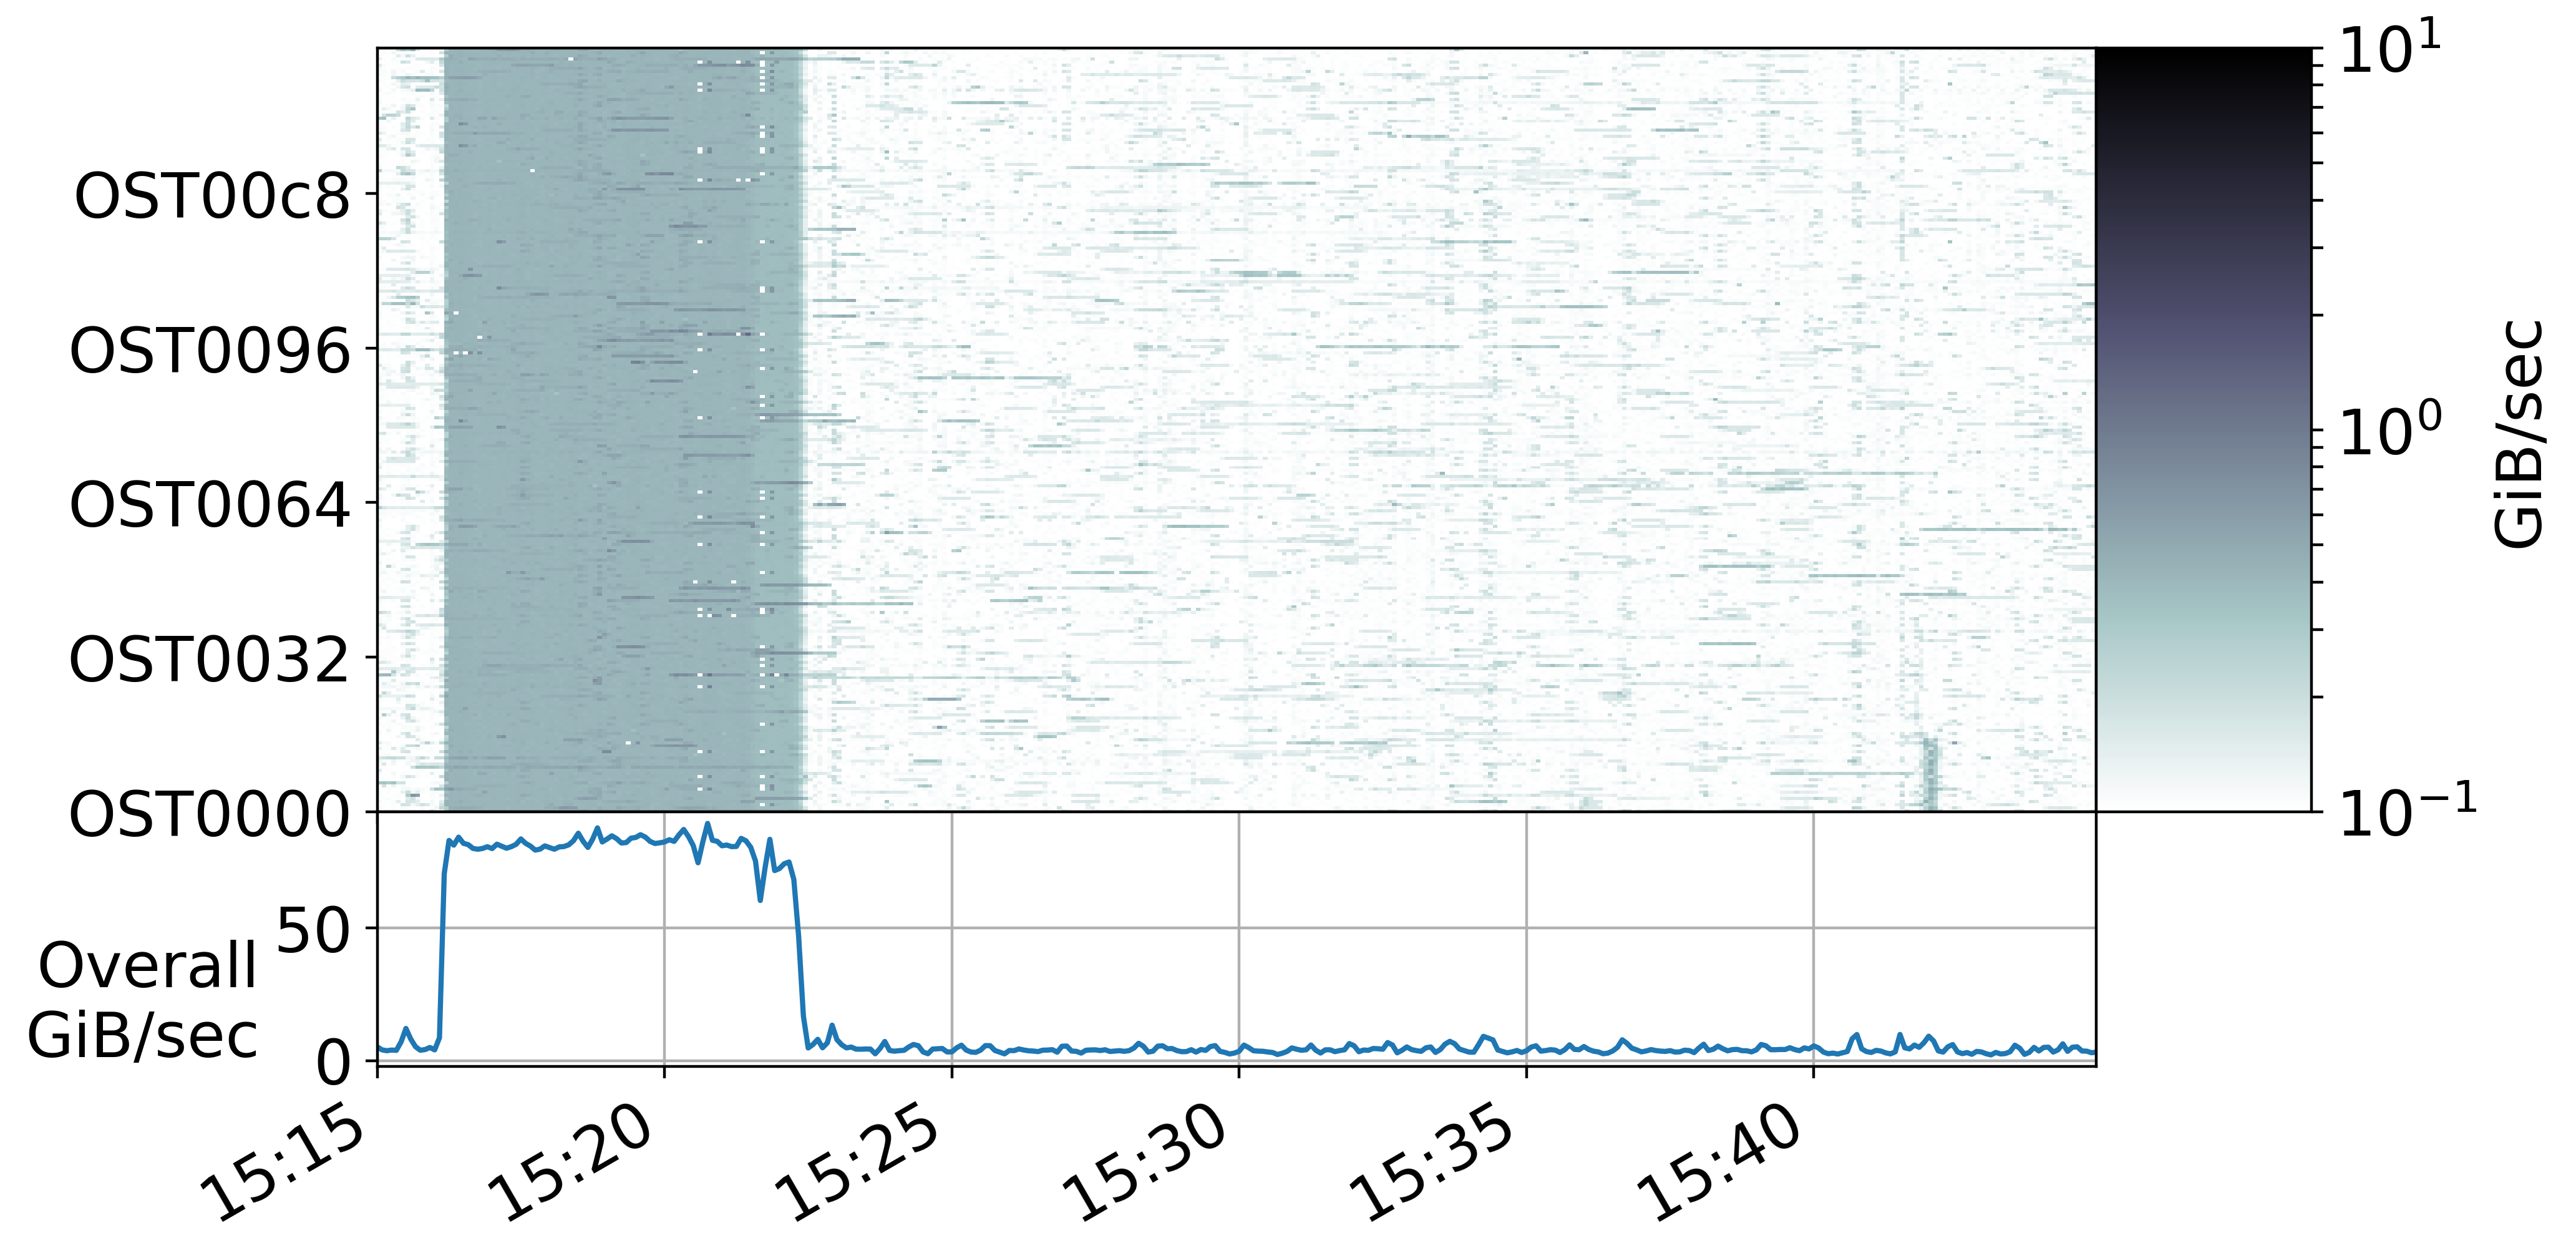
\includegraphics[width=0.9\columnwidth]{heatmap_optimized_write}
%     %\vspace{-.3in}
%     \caption{Write rate observed across all 248 OSTs on Cori's scratch file system during DataWarp stage out operations.
%     Top pane shows a naive stage-out operation where the eight files being staged out were copied to a directory with the default stripe width of 1.
%     Bottom pane shows stage-out operation after the output directory was correctly striped.}
%     \label{fig:stageout-unopt}
%     \vspace{-.2in}
% \end{figure}

\subsection{Analysis for systems planning} \label{sec:results/planning}

\TODO{long-term LMT, burst buffer, etc}

